\documentclass[
10pt,
a4paper,
openany,
svgnames,
]{book}

\usepackage[utf8]{inputenc}
\setcounter{secnumdepth}{2}
\setcounter{tocdepth}{1}

\usepackage{geometry}
\geometry{margin=1in}
\usepackage{graphicx}
\usepackage[parfill]{parskip}
\usepackage{booktabs}
\usepackage{array}
\usepackage{enumitem}
\usepackage{verbatim}
\usepackage{subfig}
\usepackage{colortbl}

%%% HEADERS & FOOTERS
\usepackage{fancyhdr} % This should be set AFTER setting up the page geometry
\pagestyle{fancy} % options: empty , plain , fancy
\renewcommand{\headrulewidth}{1pt} % customise the layout...
\renewcommand{\footrulewidth}{1pt}
\lhead{\rightmark}\chead{}\rhead{}
\lfoot{ME 310: Mechanical Design I}\cfoot{\thepage}\rfoot{S. Akamphon}

%%% ToC (table of contents) APPEARANCE
\usepackage[numbib]{tocbibind} % Put the bibliography in the ToC
\usepackage[titles,subfigure]{tocloft} % Alter the style of the Table of Contents

\usepackage{newpxtext}
\usepackage{newpxmath}
\usepackage[nointegrals]{wasysym}
\usepackage{hyperref}
\hypersetup{
    colorlinks,
    citecolor=black,
    filecolor=black,
    linkcolor=blue,
    urlcolor=blue,
}

\let\openbox\relax
\usepackage{amsthm}
\newcommand\bmmax{0}
\usepackage{bm}
\usepackage{amssymb}
\usepackage{array}
\usepackage{cleveref}
\usepackage{siunitx}

% convert engineering format to x 10^n
%\DeclareDocumentCommand{\pynum}{ m }{  \py{'\\num{'+str('{:.2e}'.format(#1))+'}'}}

\usepackage[gobble=auto]{pythontex}

%% Chapter Heading %%%%%
\usepackage[explicit]{titlesec}

%% Drawing pics with tikz %%%
\usepackage{tikz}
\usetikzlibrary{arrows,calc,decorations,shapes,decorations.pathmorphing,patterns}
\tikzset{>=latex}
\usepackage{pgfplots}
\usepackage{tikz-3dplot}
\newcommand{\AxisRotator}[1][rotate=0]{%
    \tikz[x=0.25cm,y=0.60cm,line width=.2ex,-stealth,#1] \draw(0,0) arc (150:-150:1 and 1);%
}

\definecolor{lightblue}{RGB}{180,220,255}
\definecolor{titlepagecolor}{cmyk}{1,.60,0,.40}
\definecolor{namecolor}{cmyk}{1,.50,0,.10}
\usepackage{multirow}
\usepackage{smartdiagram}

\titleformat{\chapter}
{\huge\bfseries}
{}{0pt}
{
    \begin{tikzpicture}[remember picture,overlay]
        \node[yshift=-3cm] at (current page.north west)
    {\begin{tikzpicture}[remember picture,overlay]
        \path[fill=lightblue] (0,0) rectangle (\paperwidth,3cm) ;
        \node[anchor=east,xshift=.9\paperwidth,rectangle,rounded corners=5pt,inner sep=11pt,fill=RoyalBlue]{\color{white}#1};
        \node[right, xshift=1cm]{\scalebox{4}{\Huge\thechapter}};
    \end{tikzpicture}};
    \end{tikzpicture}
}

\titleformat{name=\chapter,numberless}
{\huge\bfseries}
{}{0pt}
{\begin{tikzpicture}[remember picture,overlay]
    \node[yshift=-3cm] at (current page.north west)
    {\begin{tikzpicture}[remember picture,overlay]
        \path[fill=lightblue] (0,0) rectangle (\paperwidth,3cm) ;
        \node[anchor=east,xshift=.9\paperwidth,rectangle,rounded corners=5pt,inner sep=11pt,fill=RoyalBlue]{\color{white}#1};
      \end{tikzpicture}};
  \end{tikzpicture}
}

\titlespacing*{\chapter}{0pt}{50pt}{-10pt}

%% Section Heading %%%%%

\titleformat{\section}
{\Large\bfseries}
{}{0pt}
{\begin{tikzpicture}
    \node[fill=lightblue, rectangle, minimum height=1.5cm, minimum width=\textwidth](A){};
    \node at (A.west) [fill=RoyalBlue, anchor=west]{\color{white}\thesection\quad#1};
  \end{tikzpicture}
}

\titleformat{name=\section, numberless}
{\Large\bfseries}
{}{0pt}
{\begin{tikzpicture}
    \node[fill=lightblue, rectangle, minimum height=1.5cm, minimum width=\textwidth](A){};
    \node at (A.west) [fill=RoyalBlue, anchor=west]{\color{white}#1};
  \end{tikzpicture}
}

\titlespacing*{\section}{0pt}{20pt}{-10pt}

%% Subsection Heading %%%%

\titleformat{\subsection}
{\large\color{RoyalBlue}\bfseries}
{\thesubsection}{10pt}{#1}

%%% New column type
\newcolumntype{L}[1]{>{\raggedright\let\newline\\\arraybackslash\hspace{0pt}}m{#1}}
\newcolumntype{C}[1]{>{\centering\let\newline\\\arraybackslash\hspace{0pt}}m{#1}}
\newcolumntype{R}[1]{>{\raggedleft\let\newline\\\arraybackslash\hspace{0pt}}m{#1}}

%%% Example environment
\usepackage{thmtools}
\usepackage{mdframed}
\usepackage{float}
\declaretheoremstyle[
spaceabove=6pt, spacebelow=6pt,
headfont=\normalfont\bfseries,
notefont=\mdseries, notebraces={(}{)},
bodyfont=\normalfont,
postheadspace=1em,
numberwithin=chapter,
preheadhook={\begin{mdframed}[backgroundcolor=lightblue,
    innertopmargin=6pt , splittopskip=\topskip, %
    skipbelow= 0pt, skipabove=6pt, %
    topline=false,bottomline=false,leftline=false,rightline=false] \sloppy},
  postfoothook=\end{mdframed},
headpunct={}
]{exstyle}
\declaretheoremstyle[
spaceabove=6pt, spacebelow=6pt,
headfont=\normalfont\bfseries,
notefont=\mdseries, notebraces={(}{)},
bodyfont=\normalfont,
postheadspace=1em,
preheadhook={\begin{mdframed}[backgroundcolor=lightblue,
    innertopmargin =6pt , splittopskip = \topskip, %
    skipbelow=6pt, skipabove=0pt, %
    topline=false,bottomline=false,leftline=false,rightline=false] \sloppy},
  postfoothook=\end{mdframed},
headpunct={},
numbered=no
]{solstyle}
\declaretheorem[style=exstyle]{example}
\declaretheorem[style=solstyle]{solution}

% New list for exercises
\newlist{exercises}{enumerate}{2}
\setlist[exercises]{%
  label=\textbf{\thechapter-\arabic*}~,  % Label: Exercise C.E
  ref=\thechapter-\arabic*, % References: C.E (important!)
  align=left,               % Left align labels
  labelindent=0pt,          % No space betw. margin of list and label
  leftmargin=0pt,           % No space betw. margin of list and following lines
  itemindent=!,             % Indention of item computet automatically
}

\newcommand{\exercise}{%
\item \label{lab:\arabic{chapter}-\arabic{exercisesi}}  % Append label to item
}

\newlist{evensolution}{enumerate}{2}
\setlist[evensolution]{label=\textbf{\arabic{section}-\theevensolutioni}}
\makeatletter
\renewcommand\theevensolutioni{\@arabic{\numexpr2*\value{evensolutioni}}}
\makeatother

\SetLabelAlign{parright}{\parbox[t]{\labelwidth}{\raggedleft#1}}

\setlist[description]{style=multiline,leftmargin=5cm,font=\bfseries,%
    align=parright}

% New decoration for screws
\tikzset{/pgf/decoration/.cd,
    head width/.initial=6pt,
    head length/.initial=1.5pt,
    thread separation/.initial=1.0pt,
    thread amplitude/.initial=0.5pt,
    screw radius/.initial=1.2pt,
}
% definition of the decoration
\pgfdeclaredecoration{screw}{initial}
{
  \state{initial}[width=\pgfkeysvalueof{/pgf/decoration/head length},%
  next state=midd]
  {
    \def\headlength{%
      \pgfkeysvalueof{/pgf/decoration/head length}%
    }
    \def\headwidth{%
      \pgfkeysvalueof{/pgf/decoration/head width}%
    }
    \def\screwradius{%
      \pgfkeysvalueof{/pgf/decoration/screw radius}%
    }
    % First line
    \pgfpathlineto{\pgfpoint{0.0pt}{\headwidth/2}}
    \pgfpathlineto{\pgfpoint{\headlength}{\headwidth/2}}
    \pgfpathlineto{\pgfpoint{\headlength}{\screwradius}}
    % Second line
    \pgfpathmoveto{\pgfpoint{0.0pt}{0.0pt}}
    \pgfpathlineto{\pgfpoint{0.0pt}{-\headwidth/2}}
    \pgfpathlineto{\pgfpoint{\headlength}{-\headwidth/2}}
    \pgfpathlineto{\pgfpoint{\headlength}{-\screwradius}}
  }
  \state{midd}[width=\pgfkeysvalueof{/pgf/decoration/thread separation}*2]
  {
    \def\threadseparation{%
      \pgfkeysvalueof{/pgf/decoration/thread separation}%
    }
    \def\threadamplitude{%
      \pgfkeysvalueof{/pgf/decoration/thread amplitude}%
    }
    \def\screwradius{%
      \pgfkeysvalueof{/pgf/decoration/screw radius}%
    }
    % First line
    \pgfpathmoveto{\pgfpoint{0pt}{\screwradius}}
    \pgfpathlineto{\pgfpoint{0.5*\threadseparation}{\screwradius+\threadamplitude}}
    \pgfpathlineto{\pgfpoint{1.0*\threadseparation}{\screwradius}}
    \pgfpathlineto{\pgfpoint{1.5*\threadseparation}{\screwradius-\threadamplitude}}
    \pgfpathlineto{\pgfpoint{2.0*\threadseparation}{\screwradius}}
    % Second line
    \pgfpathmoveto{\pgfpoint{0pt}{-\screwradius}}
    \pgfpathlineto{\pgfpoint{0.5*\threadseparation}{-\screwradius-\threadamplitude}}
    \pgfpathlineto{\pgfpoint{1.0*\threadseparation}{-\screwradius}}
    \pgfpathlineto{\pgfpoint{1.5*\threadseparation}{-\screwradius+\threadamplitude}}
    \pgfpathlineto{\pgfpoint{2.0*\threadseparation}{-\screwradius}}
    % Thread
    \pgfpathmoveto{\pgfpoint{0.5*\threadseparation}{\screwradius+\threadamplitude}}
    \pgfpathlineto{\pgfpoint{1.5*\threadseparation}{-\screwradius+\threadamplitude}}
  }
  \state{final}
  {
    \def\screwradius{%
      \pgfkeysvalueof{/pgf/decoration/screw radius}%
    }
    %\pgfpathlineto{\pgfpointdecoratedpathlast}
    \pgfpathmoveto{\pgfpoint{0pt}{\screwradius}}
    \pgfpathlineto{\pgfpoint{\screwradius/2}{0pt}}
    \pgfpathlineto{\pgfpoint{0pt}{-\screwradius}}
  }
}

%% bibliography %%%%

\usepackage[style=numeric,backend=biber]{biblatex}
\addbibresource{me310-2.bib}% chktex 8

%%% END Article customizations

%%% The "real" document content comes below...

%%%%%%%%%%%%%%%%%%%%%%%%%%%%%%%%%%%%%%%%%%%%%%%%%%%%%%%%%%%%%%%%%%%%%%%%%%%%%%%%%%%%%%%%%%%%%%%%%%%%%%%%%%%%%%%%%%%%%%%%%%%%%%%%%%%%%%%%%%%%%%%%%%%%%%%%%%%%%%%%%%%%%%%%%%%%%%

\begin{document}

\frontmatter

%\maketitle
\begin{titlepage}
  \newgeometry{top=1cm,left=1cm} %defines the geometry for the titlepage
  \pagecolor{titlepagecolor}
  \includegraphics[scale=0.2]{pictures/logo-tu} \\
  \noindent
  \color{white}
  \makebox[0pt][l]{\rule{1.3\textwidth}{1pt}}
  \par
  \noindent
  \textbf{\textsf{Thammasat University}} \textcolor{namecolor}{\textsf{Faculty of Engineering}}
  \vfill
  \hspace{1cm}
  \includegraphics[scale=0.23]{pictures/tube-connection}
  \vfill
  \noindent
  \raggedleft{\Huge {ME 310: Mechanical Design}} \\
  \vspace{1cm}
  \raggedleft{\LARGE {Part II:\ Power Transmission}} \\
  \vspace{1cm}
  \noindent
  {\Large {Sappinandana Akamphon}}
\end{titlepage}

\restoregeometry% restores the geometry
\nopagecolor% Use this to restore the color pages to white

\chapter*{Preface}

This book is the second part of ME 310: Mechanical Design. In this book, power transmission components are covered.

\vspace{2cm}\hspace{10cm} Sappinandana Akamphon

\chapter*{Revisions}

\paragraph{September 2019}

Start of Mechanical Design Part II.\

\tableofcontents

\listoffigures

\listoftables

\mainmatter{}

\chapter{Shaft and Shaft Components}

Most engineering systems are powered by rotational machinery such as internal combustion engines and electrical motors. It is, thus, extremely important that we understand and properly design power tranmission mechanism from the rotational machinery power source to intended components. Shafts remains one of the most prevalent methods of transmitting rotational power, and so it is our first chapter into the world of power transmission design.

By itself, shaft design is no more complex than other components under static or cyclic loadings already covered in the first book of this series. However, as shafts lie at the heart of most machine design applications, its final design will also depend on the design of other components that are to be mounted or connected to the shaft.

\section{Shaft Materials}

There are two main concerns with designing a shaft: deflection and strength. Deflection is not affected by material strength. In fact, it depends only on the stiffness, represented by the Young's modulus. Since the Young's modulus is essentially the same for all steels, material choice matters little for deflection.

Strength, on the other hand, constitute a major concern for shaft design. Strength is necessary to resist loading stresses and fatigue stresses from the constant rotation. Many shafts are made from low carbon, cold-drawn or hot-rolled steel such as ANSI 1020-1050 steels. Significant strengthening from heat treatment or high alloy is often not neeeded. And fatigue failure is only reduced moderately by increase in strength, after a certain level notch sensitivity begins to counteract its benefit.

A good way to select a proper shaft material is to start with an inexpensive low or medium carbon steel for the first round of calculations. If strength considerations turn out to be the limiting factor over deflection, select a higher strength material and reduce the shaft size accordingly until deflection becomes an issue. The cost of the material and its manufacturing processes must be weighed against the need for smaller shaft diameter.

When additional strengthening is needed, typical alloy steels for heat treatment include ANSI 340-50, 3140-50, 4140, 4340, 5140, and 8650. Shafts don't usually need surface hardening unless there is significant risk of wear from journal bearing, in which case surface hardening include carburizing grades of ANSI 1020, 4320, 4820, and 8620. \cite{shigley2011shigley}

\section{Shaft Layout}

Generally a shaft is a cylinder with segments of varying cross sections to accommodate components like gears, bearings, pulleys, etc. Shaft shoulders are normally used to axially locate elements and to take any axial thrust loads. \Cref{fig: worm-gear speed reducer layout} illustrates the cross-section of a vertical worm-gear speed reducer. In this figure, the shaft steps are used to axially locate the two tapered bearings and the spur gear.

\begin{figure}[H]
  \centering
  \includegraphics[height=0.3\textheight]{pictures/Shafts/speed-reducer-layout}
  \caption{A vertical worm-gear speed reducer. \emph{(Courtesy of the Cleveland Gear Company.)}}
  \label{fig: worm-gear speed reducer layout}
\end{figure}

\subsection{Axial Layout of Components}

The axial positioning of components is often preset by the layout of the housing and other meshing components. Generally it is advisable to support any loading-carrying components between bearings. (TODO: NEED FIGURE) However, pulleys and sprockets tend to be mounted outside of the bearing pairs for ease of installation of the belt or chain. The length of the shaft should be kept as short as possible to minimize deflection and resultant load on the bearings.

In most cases, a shaft will only require two bearings, but in cases with long shafts carrying multiple load-carrying components, it may be necessary to use more than two bearings for additional support. In such a case, particular care must be given to the alignment of the bearings.

\subsection{Supporting Axial Loads}

There are use cases where axial loads in shaft may be significant, in which case it is important to provide a means to transfer the axial loads into the shaft. The shaft would then transfer the loads to a bearing and to the ground. This is necessary for shafts mounted with components that generate axial loads like bevel and helical gears, or tapered roller bearings.

It is usually sufficient to have only one bearing carry the axial load. This allows for greater tolerances on shaft length dimensions and prevents binding from shaft thermal expansions, which is especially significant in long shafts. TODO: figures showing shaft that carries axial loads.

\subsection{Support for Torque Transmission}

Most shafts serve to transfer torque from an input (gear, pulley, engine, motor, etc.) to an output gear or pulley. The shaft must be sized to support torsional stress and its resultant angle of twist. It is also important to provide a way to transmit the torque between the gear (or pulley) and the shaft itself. Common torque transfer methods are:

\begin{itemize}
\item Keys
\item Splines
\item Setscrews
\item Pins
\item Press or shrink fits
\item Tapered fits
\end{itemize}

There are also shafts that are designed to fail if excessive torque is applied, to prevent failure of more expensive components. Details of the components and their design process is covered in \cref{sec: torque transmission components}.

\section{Shaft Design for Stress}

It is not always necessary to evaluate stresses at every point; the same goes for shafts as well. Only a few potentially critical locations should be more than enough. Since the main types of load on shafts are torsion and bending, it follows that most critical locations on the shafts are on the outer surface--typically where the bending moment is large, the torque is large, and where stress concentrations exist.

In order to determine the bending moments, torques, and shear forces on a shaft, it is usually a good idea to draw shear and bending moment diagrams. Since most shafts are loaded by gears and pulleys, introducing forces in two planes, two diagrams are needed to determine the loads. Resultant moments can be obtained simply by adding the moments as vectors at points of interest. The normal stress due to bending will be highest on the outer surfaces and will contribute to fatigue on a rotating shaft.

Axial stresses on shafts from axial loads caused by helical gears or tapered roller bearings are typically negiligible compared to the bending stress. The axial stresses are also usually constant, meaning that they rarely contribute significantly to fatigue. However, axial stresses resulting from axial loads applied through other means should be explicitly considered.

Let us now consider the shaft stresses, which are usually the combination of normal stresses from bending and axial stresses, and shear stress from torsion.

\begin{align}
  \label{eq: shaft normal and shear stresses}
  \begin{array}{ll}
    \sigma_a = K_f \dfrac{M_a y}{I} & \sigma_m = K_f \dfrac{M_m y}{I} \\[1em]
    \tau_a = K_{fs} \dfrac{T_a r}{J} & \tau_m = K_{fs} \dfrac{T_m r}{J}
  \end{array}
\end{align}

If we assume a solid shaft with circular cross section, we can further simplify the expression to

\begin{align}
  \label{eq: shaft normal and shear stresses simplify}
  \begin{array}{ll}
    \sigma_a = K_f \dfrac{32M_a}{\pi d^3} & \sigma_m = K_f \dfrac{32M_m}{\pi d^3} \\[1em]
    \tau_a = K_{fs} \dfrac{16T_a}{\pi d^3} & \tau_m = K_{fs} \dfrac{16T_m }{\pi d^3}
  \end{array}
\end{align}

The stresses can be combined into stress amplitude and average stress using maximum distortion energy theory (MDET or von Mises) as

\begin{align}
  \label{eq: von mises shaft stress}
  \sigma_{ae} &= \left( \sigma_a^2 + 3\tau_a^2 \right)^{1/2} = \left[ \left( \dfrac{32 K_fM_a}{\pi d^3} \right)^2 + 3\left( \dfrac{16 K_{fs} T_a}{\pi d^3} \right)^2 \right]^{1/2} \\
  \sigma_{me} &= \left( \sigma_m^2 + 3\tau_m^2 \right)^{1/2} = \left[ \left( \dfrac{32 K_fM_m}{\pi d^3} \right)^2 + 3\left( \dfrac{16 K_{fs} T_m}{\pi d^3} \right)^2 \right]^{1/2}
\end{align}

The stress concentration factors for the average stress component in ductile materials can sometimes be ignored since the materilas can yield locally at the discontinuity.

These equivalent stresses can be evaluated in design equations to determine the safety factor $N_s$ or the required diameter $d$ using the the modified Goodman diagram as

\begin{align*}
  \frac{1}{N_s} = \frac{\sigma_{ae}}{S_e} + \frac{\sigma_{me}}{S_{ut}}
\end{align*}

Substituting for $\sigma_{ae}$ and $\sigma_{me}$ results in

\begin{align*}
  \frac{1}{N_s} = \frac{16}{\pi d^3} \left\{ \frac{1}{S_e} \left[ 4 \left( K_f M_a \right)^2 + 3 \left( K_{fs} T_a \right)^2 \right]^{1/2} + \frac{1}{S_{ut}} \left[ 4 \left( K_f M_m \right)^2 + 3 \left( K_{fs} T_m \right)^2 \right]^{1/2} \right\}
\end{align*}

The required diameter $d$ can be solved from the previous equation as

\begin{align*}
  d = \left( \frac{16N_s}{\pi} \left\{ \frac{1}{S_e} \left[ 4 \left( K_f M_a \right)^2 + 3 \left( K_{fs} T_a \right)^2 \right]^{1/2} + \frac{1}{S_{ut}} \left[ 4 \left( K_f M_m \right)^2 + 3 \left( K_{fs} T_m \right)^2 \right]^{1/2} \right\} \right)^{1/3}
\end{align*}

In many applications, rotating shafts will be under constant bending and torsion, resulting in completely reverse bending stress ($M_m = 0$) and constant torsional shear stress ($T_a = 0$). This means the required diameter becomes

\begin{align*}
  d = \left( \frac{16N_s}{\pi} \left\{ \frac{2 K_f M_a}{S_e} + \frac{\sqrt{3} K_{fs} T_m}{S_{ut}} \right\} \right)^{1/3}
\end{align*}

\begin{example} Size the shaft (AISI 1040, $S_{y}$ = 400 MPa, $S_{ut}$ = 600 MPa) using
  \begin{enumerate}
    \item MDET
    \item Soderberg theory
  \end{enumerate}

  so that the safety factor $N_{s}$ = 3.
\end{example}
\begin{solution} \hfill
  \begin{enumerate}
    \item MDET: The torque loaded on the pulley by the belt is

      \begin{pycode}
        from math import *
        F1 = 20
        F2 = 2020
        F = F1+F2
        rpulley = 0.1
        L = 0.6
        T = (F2 - F1)*rpulley
        K_f = 2.14
        K_fs = 3
        sigma = K_f*4*(F1+F2)*L/4/pi
        tau = K_fs*2*T/pi
        sigma_e = sqrt(sigma**2 + 3*tau**2)
        S_y = 4e8
        S_ut = 6e8
        N_s = 3
        r_mdet = (N_s*sigma_e/S_y)**(1/3)
        sigma_a = sigma
        sigma_m = 0
        tau_a = 0
        tau_m = tau
        sigma_ae = sqrt(sigma_a**2 + 3*tau_a**2)
        sigma_me = sqrt(sigma_m**2 + 3*tau_m**2)
        r_sod = (N_s*(sigma_ae/(0.5*S_ut) + sigma_me/S_y))**(1/3)
      \end{pycode}
      \begin{align*}
        T &= (\py{F2} - \py{F1})(\py{rpulley}) \\
          &= \py{T} \text{ N-m}
      \end{align*}

      There is also \py{F2 + F1} N of force pulling at the pulley due to the combined belt tension. The torque generates shear stress throughout the shaft, with the maximum value at the surface. The belt tension creates bending stresses, whose maximum values are are the top and bottom of the shaft at the middle. This means that the critical points on the shaft (without considering stress concentration from the key/keyseat) are at the top and bottom of the shaft at the middle. In this problem, we will take the bottom of the shaft at the middle. The stress concentration of the keyseat is taken to be $K_{f}$ = 2.14 in bending and $K_{fs}$ = 3.0 in torsion.

      \begin{align*}
        \sigma &= K_{f}\frac{My}{I} = (\py{K_f})\frac{\py{F}(\py{L})(r)}{4 \pi r^{4}/4} \\
               &= \frac{\py{round(sigma)}}{r^{3}} \text{ Pa} \\
        \tau &= K_{fs}\frac{Tr}{J} = (\py{K_fs})\frac{\py{T}(r)}{\pi r^{4}/2} \\
               &= \frac{\py{round(tau)}}{r^{3}} \text{ Pa}
      \end{align*}

      We can then combine them using MDET to obtain the equivalent stress $\sigma_{e}$.

      \begin{align*}
        \sigma_{e} &= \sqrt{ \sigma^{2} + 3 \tau^{2} } \\
                   &= \sqrt{ \left( \frac{\py{round(sigma)}}{r^{3}} \right)^{2} + 3 \left( \frac{\py{round(tau)}}{r^{3}} \right)^{2} } \\
        N_{s} &= \frac{S_{y}}{\sigma_{e}} \\
        3 &= \frac{400 \times 10^{6} r^{3}}{\py{round(sigma_e)}} \\
        r &= \py{round(r_mdet,4)} \text{ m}
      \end{align*}

    \item Soderberg: using the criteria, we must calculate the minimum and maximum bending moments and torques, which will then be used to determine the stress amplitudes and average stresses. We already determine the maximum bending moment and torque, which we used to determine the corresponding stresses for MDET. We now only need to find out the minimum bending moment and torque. The minimum bending moment occurs when the shaft rotates by half a revolution, for which the beam willbe under a compressive stress of the same magnitude.
      \begin{align*}
        \sigma_{\min} &= -\frac{\py{round(sigma)}}{r^{3}} \\
        \sigma_{a} &= \frac{\sigma_{\max} - \sigma_{\min}}{2} \\
                      &= \frac{\py{round(sigma)}}{r^{3}}
      \end{align*}
      If the shaft is under continuous operation, the applied torque is constant, which means that the torque amplitude $T_{a}$ = 0 and the average torque $T_{m} = T$. We can plug this into the sequation to determine equivalent amplitude and average stresses.
      \begin{align*}
        \sigma_{ae} &= \sqrt{ \sigma_{a}^{2} + 3 \tau_{a}^{2} } = \frac{\py{round(sigma_ae)}}{r^{3}} \\
        \sigma_{me} &= \sqrt{ \sigma_{m}^{2} + 3 \tau_{m}^{2}} = \frac{\py{round(sigma_me)}}{r^{3}} \\
        %\frac{1}{3} &= \frac{\py{round(sigma_ae)}}{0.5(\pynum{S_ut})r^{3}} + \frac{\py{round(sigma_me)}}{\pynum{S_y}r^{3}} \\
        r &= \py{round(r_sod,4)} \text{ m}
      \end{align*}
  \end{enumerate}
\end{solution}

\begin{example} Using the settings from the previous example, redetermine the shaft size if the maximum operating speed is 10000 rpm.

  \begin{pycode}
    E = 210e9
    omega_max = 10000
    omega_rad = omega_max * 2*pi/60
    rho = 7800
    r = N_s*omega_rad*L**2 / pi**2 * sqrt(4 * rho/E)
  \end{pycode}


\end{example}
\begin{solution}
  For a simply supported shaft, the first natural frequency that can cause shaft whirling is

  \begin{align*}
    \omega_{1} = \left( \frac{\pi}{l} \right)^{2} \sqrt{ \frac{EI}{A \rho} }
  \end{align*}

  We must first convert the angular velocity into rad/s: 10000 rpm = 10000 * 2$\pi$/60 = \py{round(omega_rad)} rad/s. To achieve the safety factor of 3, the first natural frequency of the shaft must be

  \begin{align*}
    %\omega_{1} &= \py{N_s}(\py{round(omega_rad)}) = \left( \frac{\pi}{\py{L}} \right)^{2} \sqrt{ \frac{\pynum{E} \pi r^{4}/4 }{\pi r^{2} \rho}} \\
    r &= \py{round(r,3)} \text{ m}
  \end{align*}
  The designed shaft has to follow the largest shaft that satisfy each of the condition, therefore the required radius is 4.4 cm.
\end{solution}

\section{Torque Trasmission Components} \label{sec: torque transmission components}

\chapter{Journal Bearings and Lubrication}

\section*{Overview of Bearings}
\label{sec:org555f498}

\subsection*{What are bearings?}
\label{sec:orgfea7d47}
\begin{itemize}
\item A feature that allows relative motions between components
\begin{itemize}
\item Linear motions
\item Rotary motions
\end{itemize}
\end{itemize}

\subsection*{Two types of bearings}
\label{sec:org98f6af3}

\begin{itemize}
\item Contact: sliding or rolling

\item Non-contact: fluid film or magnetic
\end{itemize}

\section*{Contact Bearings}
\label{sec:org1d69975}

\subsection*{Sliding Contact Bearings}
\label{sec:orgd75a2e1}

\begin{itemize}
\item Commonly used in low- to medium-speed applications
\end{itemize}

\begin{center}
%\includegraphics[width=.9\linewidth]{./pictures/sliding-contact-bearing.jpg}
\end{center}

\begin{itemize}
\item Lubrication is used to reduce wear and friction
\end{itemize}

\subsection*{Materials for Sliding Contact Bearing}
\label{sec:org6549bb0}

\begin{itemize}
\item Typically hard materials (shaft) on soft (bearing)
\item Materials:
\begin{itemize}
\item Polymers: nylon is king!
\item Brass
\item Ceramics
\end{itemize}
\item Check on bearing stress
\item Aluminum-on-aluminum is a no-no
\end{itemize}

\subsection*{Bearing Contact Pressure}
\label{sec:orgfbd15a0}

\begin{align*}
    P &= \frac{F}{DL} \\
    P_{\max} &= \frac{4}{\pi} \frac{F}{DL}
 \end{align*}

\subsection*{PV Factor}
\label{sec:org3e1ac8b}

\begin{itemize}
\item pressure \(\times\) velocity
\item tradeoff in choosing bearing materials
\item higher pressure \(\rightarrow\) low speed, and vice versa
\end{itemize}

\subsection*{PV Table for Metals}
\label{sec:orgb26b2cd}

\begin{center}
%\includegraphics[width=.9\linewidth]{./pictures/pv-metal.png}
\end{center}

\subsection*{PV Table for Nonmetals}
\label{sec:org7bf1135}

\begin{center}
%\includegraphics[width=.9\linewidth]{./pictures/pv-nonmetal.png}
\end{center}

\subsection*{Example: Sleeve Bearing for a Low-speed Shaft}
\label{sec:org45b86ce}

A 30-cm long shaft whose diameter \(D\) is 3 cm is operated at 1000 rpm. The shaft has a spur gear whose \(R_{\text{pitch}}\) = 10 cm mounted in the middle with a bearing at each end. The gear is transferring the power of 1.5 kW. The gear has pressure vessel \(\theta\) = 20\(^{\circ}\). Determine the minimum bearing length \(L\) using nylon.

\subsection*{Solution}
\label{sec:orgdf72955}

First, let us determine the force on the bearing. Since spur gears don't generate any axial load, the forces will simply be the radial + tangential load, perpendicular to the shaft.

\begin{align*}
    T &= \frac{P}{\omega} \\
      &= \frac{1500}{1000(2\pi / 60)} = 14.3 \text{ N-m} \\
    F &= \frac{T}{R_{\text{pitch}} \cos \theta} \\
      &= \frac{14.3}{0.1 \cos 20^{\circ}} = 152 \text{ N} \\
\end{align*}

\subsection*{Solution}
\label{sec:orgbf73358}

Since the gear is mounted in the middle, the force on each bearing is half of the force.

\begin{align*}
    F_{bearing} = \frac{152}{2} = 76 \text{ N}
\end{align*}

We can't determine the bearing pressure yet since we don't know the bearing length. We can determine the surface velocity, however.

\begin{align*}
    v = \omega (D/2) = 1000 (2\pi / 60) (0.03/2) = 1.57 \text{ m/s}
\end{align*}

\subsection*{Solution}
\label{sec:org15bf95d}

We double-check that \(v < V_{nylon} (1.57 < 3.0)\) so nylon is an acceptable choice. The length of bearing, then should be

\begin{align*}
    P_{bearing}v &< (PV)_{nylon} \\
    \frac{F_{bearing}}{DL}v &< 0.11 \times 10^6 \\
    \frac{76}{0.03L} 1.57 &< 1.1 \times 10^5 \\
    L &> 0.036 = 3.6 \text{ cm}
\end{align*}

%%%%%%%%%%%%%%%%%%%%%%%%%%%%%%%%%%%%%%%%%%%%%%%%%%%%%%%%%%%%%%%%%%%%%%%%%%
%%%%%%%%%%%%%%%%%%%%%%%%%%%%%%%%%%%%%%%%%%%%%%%%%%%%%%%%%%%%%%%%%%%%%%%%%%
%%%%%%%%%%%%%%%%%%%%%%%%%%%%%%%%%%%%%%%%%%%%%%%%%%%%%%%%%%%%%%%%%%%%%%%%%%
%%%%%%%%%%%%%%%%%%%%%%%%%%%%%%%%%%%%%%%%%%%%%%%%%%%%%%%%%%%%%%%%%%%%%%%%%%

\chapter{Rolling-Contact Bearings}

\section*{Rolling Contact Bearings}
\label{sec:org223e543}

\subsection*{Rolling Elements}
\label{sec:orgda844f8}
\begin{itemize}
\item suitable for medium- to high-speed applications
\item use balls or rollers to avoid friction
\end{itemize}

\subsection*{Rolling Element Types}
\label{sec:orgf0733bc}

\begin{center}
%\includegraphics[width=.9\linewidth]{./pictures/ball-bearing.jpg}
\end{center}
\begin{center}
%\includegraphics[width=.9\linewidth]{./pictures/roller-bearing.jpg}
\end{center}
\begin{center}
%\includegraphics[width=.9\linewidth]{./pictures/needle-roller-bearing.jpg}
\end{center}

\subsection*{Bearing Series}
\label{sec:orgc9e647d}

\begin{center}
%\includegraphics[width=.9\linewidth]{./pictures/bearing-series.png}
\end{center}

\subsection*{Bearing Table}
\label{sec:org54e4707}

\begin{center}
%\includegraphics[width=.9\linewidth]{./pictures/bearing-table.png}
\end{center}

\subsection*{Bearing Life Requirement}
\label{sec:org689594f}

\begin{align*}
    L &= L_R K_r \left( \frac{C}{F_e} \right)^{10/3} \\
    C &= F_e \left( \frac{L}{K_r L_R} \right)^{0.3}
\end{align*}

\begin{center}
\begin{tabular}{ll}
\(L\) & life corresponding to equivalent load \(F_e\)\\
\(L_R\) & life corresponding to rated capacity = 9 \(\times\) 10\(^7\) rev\\
\(K_r\) & reliability factor\\
\(C\) & rated capacity\\
\(F_e\) & equivalent load\\
\end{tabular}
\end{center}

\subsection*{Bearing Rated Capacity}
\label{sec:org59f1f39}

\begin{center}
%\includegraphics[width=.9\linewidth]{./pictures/bearing-rated-capacity.png}
\end{center}

\subsection*{Reliability Factor}
\label{sec:org8b329d7}

\begin{center}
%\includegraphics[width=.9\linewidth]{./pictures/reliability-factor.png}
\end{center}

\subsection*{Equivalent Load}
\label{sec:org6e4ada8}

Let \(e = F_a / F_r\)

for radial ball bearings

\begin{align*}
    F_e = \left\{
    \begin{array}{ll}
        F_r & e < 0.35 \\
        F_r \left[ 1 + 1.115(e - 0.35) \right] & 0.35 < e < 10 \\
        1.176 F_a & e > 10
    \end{array}
    \right.
\end{align*}

for angular ball bearings

\begin{align*}
    F_e = \left\{
    \begin{array}{ll}
        F_r & e < 0.68 \\
        F_r \left[ 1 + 0.87(e - 0.68) \right] & 0.68 < e < 10 \\
        0.911 F_a & e > 10
    \end{array}
    \right.
\end{align*}

\subsection*{Typical Bearing Design Life}
\label{sec:org412d1a6}

\begin{center}
%\includegraphics[width=.9\linewidth]{./pictures/designed-bearing-life.png}
\end{center}

\begin{example} Radial Ball Bearing Selection
\label{sec:org7e80c97}

Select a radial ball bearing for a shaft intended for a continuous 8-hr-a-day operation at 1800 rpm with 95\% reliability. Axial and radial loads are 1.2 kN and 1.5 kN, respectively.

\end{example}

\begin{solution}
\label{sec:orgb6be1c8}

First, we need to calculated \(F_e\).

$$e = \frac{F_a}{F_r} = \frac{1.2}{1.5} = 0.8$$

 For radial ball bearing,

\begin{align*}
  F_{e} &= F_r \left[ 1 + 0.87(e - 0.68) \right] \\
        &= 1500 \left[ 1 + 1.115(0.8 - 0.35) \right] \\
        &= 2276 \text{ N}
\end{align*}

Required life for 8-hr-a-day service (assumed every day) = 30000 hrs

Life in revolutions

$$L = 1800(30000)(60) = 3.24 \times 10^9 \text{ revolutions}$$

For 95\% reliability \(K_r\) = 0.63

\begin{align*}
    C = 2276 \left( \frac{3.24 \times 10^9}{0.63 (9 \times 10^7)} \right)^{0.3} = 7661 \text{ N} = 7.66 \text{ kN}
\end{align*}

For extra-light, light, and medium series, the required bore are 55, 35, and 30 mm, respectively

The models corresponding to the bore are L11, 207, and 306, respectively.

\end{solution}


%%%%%%%%%%%%%%%%%%%%%%%%%%%%%%%%%%%%%%%%%%%%%%%%%%%%%%%%%%%%%%%%%%%%%%%%%%%%%
%%%%%%%%%%%%%%%%%%%%%%%%%%%%%%%%%%%%%%%%%%%%%%%%%%%%%%%%%%%%%%%%%%%%%%%%%%%%%
%%%%%%%%%%%%%%%%%%%%%%%%%%%%%%%%%%%%%%%%%%%%%%%%%%%%%%%%%%%%%%%%%%%%%%%%%%%%%

\chapter{Gears}

\section{Gear Overview}

\begin{frame}{Why Gears?}
  \begin{itemize}
    \item Convert high speed and low torque to that requires low speed and high torque
    \item Speed: easy to get because voltage is easy
    \item Torque: hard to get because it requires large current
  \end{itemize}
\end{frame}

\begin{frame}{Principles of Gears}
  \begin{itemize}
    \item Allow positive engagement between teetch
    \item High forces can be transmitted while in rolling contact
    \item Do not need friction to operate
  \end{itemize}
\end{frame}

\begin{frame}{Basic Law of Gearing}
  \begin{itemize}
    \item Point of contact between two mating gears is always the same relative distances from the two centers.
    \item Any gear tooth profiles that follow the law of gearing will result in constant relative speed of rotation
  \end{itemize}

  \begin{figure}[htbp]
    \centering
    %\includegraphics[width=0.7\textwidth]{pictures/gear-profile}
  \end{figure}
\end{frame}

\begin{frame}{Gear Geometry}
  \begin{figure}[htbp]
    \centering
    %\includegraphics[height=0.85\textheight]{pictures/gear-pair}
  \end{figure}
\end{frame}

\begin{frame}{Module of a Gear, $m$}
  \begin{itemize}
    \item Term used to define gear tooth size
    \item Defined as ratio of pitch diameter to number of teeth
          \begin{align*}
            m = \frac{D_{\text{pitch}}}{z}
          \end{align*}
    \item A pair of meshing gears must have the same modules!
  \end{itemize}
\end{frame}

\begin{frame}{Gear Types}
  \begin{figure}[htbp]
    \centering
    %\includegraphics[height=0.85\textheight]{pictures/gear-types}
  \end{figure}
\end{frame}

\begin{frame}{Gear Terminology}
  \begin{description}
    \item[Pinion] smaller of two gears, usually driving
    \item[Gear] Larger of the two. Also called \emph{wheel}. Usually driven.
  \end{description}
\end{frame}

\begin{frame}{Gear Materials}
  \begin{itemize}
    \item Steel: medium-carbon steel + heat treatment + grinding
    \item Cast iron: surface fatigue > bending fatigue
    \item Nonferrous: bronzes $\rightarrow$ corrosion + wear resistant, low friction
    \item Nonmetallic: Nylon $\rightarrow$ low friction and weight + corrosion resistant, but low thermal conductivity
  \end{itemize}
\end{frame}
\begin{frame}{Gear Efficiency}
  \begin{itemize}
    \item With friction, gears are 90 - 95\% efficient because of mostly rolling contact
      \begin{align*}
        T_{\text{out}} &= \frac{\eta T_{\text{in}} d_{\text{out}}}{d_{\text{in}}} \\
        \omega_{\text{out}} &= \frac{\omega_{\text{in}} d_{\text{in}}}{d_{\text{out}}} \\
        P_{\text{out}} &= T_{\text{out}} \omega_{\text{out}}
      \end{align*}
  \end{itemize}
\end{frame}

% \begin{frame}{Force on Gears and Shaft}
%   \begin{description}
%     \item[Spur] $$ F = \frac{T}{r \cos \theta}$$
%     \item[Worm and Helical] $$ F = \frac{T}{r \cos \theta \cos \alpha} $$
%   \end{description}
% \end{frame}
%
\section{Gear Trains}

\begin{frame}{Gear Trains}
  When large reduction is required
  \begin{itemize}
    \item Large gear + small pinion: simple, but large stress and interference
    \item Multiple pairs of gears and pinions: less simple, low stress, large space
    \item Planetary gears: complex, low stress, small space
  \end{itemize}
\end{frame}

\begin{frame}{Normal Gear Trains}
  \begin{figure}[htbp]
    \centering
    %\includegraphics[width=0.6\textwidth]{pictures/normal-gear-trains}
  \end{figure}
  \begin{align*}
    e_{total} &= e_{1}e_{2}\cdots \\
  \end{align*}
\end{frame}

\begin{frame}{Planetary/Epicyclic Gear Train}
  \begin{itemize}
    \item Planetary or epicyclic gears enable a high reduction ratio in small spaces
  \end{itemize}
  \begin{figure}[htbp]
    \centering
    %\includegraphics[width=0.8\textwidth]{pictures/planetary-gearbox}
  \end{figure}
\end{frame}

\begin{frame}{Planetary Gear Components}
  \begin{figure}[htbp]
    \centering
    %\includegraphics[width=0.9\textwidth]{pictures/planetary-gear-comp}
  \end{figure}
\end{frame}

\begin{frame}{Planetary Gears: Torque, Forces, and Reduction Ratios}
  \begin{itemize}
    \item Symmetry $\rightarrow$ no net force on shaft
    \item Multiple planet gears reduce individual torque/force
    \item Any combination of fixed, input, output gears
    \item 1 gear box -> multiple gear reduction ratios
  \end{itemize}
\end{frame}

% \begin{frame}{Force Analysis: Spur Gears}
%   \begin{align*}
%     F &= \frac{T}{r \cos \theta} \\
%     F_{t} &= F \cos \theta \\
%     F_{r} &= F \sin \theta \\
%   \end{align*}
% \end{frame}

\begin{example}
  % \includegraphics[width=1.1\textwidth]{pictures/planet-example}
\end{example}

\begin{solution}
  Fixed ring: \\
  \begin{align*}
    \omega_{\text{carrier}} &= 9 \\
    \omega_{\text{planet}} &= (9) \frac{60/2 + 20/2}{20/2} = 36 \\
    \omega_{\text{sun}} &= (36) \frac{20}{30} = 24 \\
    e &= 9/24 = 0.375
  \end{align*}

  \begin{table}[H]
    \centering
    \begin{tabular}{ccccc}
      \toprule
      Fixed & Input & Planet & Output & RR \\
      \midrule
      Ring & Carrier 9 & 36 & Sun 24 & 0.375 \\
      Sun & Carrier 9 & 36 & Ring 14.4 & 0.625 \\
      Carrier & Sun 9 & 27 & Ring 5.4 & 1.667 \\
      \bottomrule
    \end{tabular}
  \end{table}
\end{solution}

\section{Spur Gears}

\begin{frame}{Spur Gears}
  \begin{figure}[htbp]
    \centering
    %\includegraphics[width=0.6\textwidth]{pictures/spur-gears}
  \end{figure}
  \begin{itemize}
    \item Straight involute teeth $\rightarrow$ most common
          \begin{align*}
            F = \frac{T}{R_{\text{pitch}} \cos \theta}
          \end{align*}
    \item Lead to shaft bending
  \end{itemize}
\end{frame}

\begin{frame}{Spur Gear Stress}
  \begin{itemize}
    \item Bending Stress $\rightarrow$ AGMA stress equation
    \item Consider tooth as a cantilever beam
  \end{itemize}
  \begin{align*}
    \sigma = \frac{F_{t}}{bY_{J}m} K_{O} K_{m} K_{v}
  \end{align*}
  \begin{description}
    \item[$F_{t}$] tangential force
    \item[$b$] face width
    \item[$Y_{J}$] geometry factor
    \item[$m$] module
  \end{description}
\end{frame}

\begin{frame}{Geometry Factor: $Y_{J}$}
  \begin{figure}[htbp]
    \centering
    %\includegraphics[width=0.9\textwidth]{pictures/geometry-factor}
  \end{figure}
\end{frame}

Overload Factor: $K_{O}$
  \begin{table}[htbp]
    \centering
    \begin{tabular}{lcccc}
      \toprule
      \multirow{2}{3cm}{Power source} & \multicolumn{4}{c}{Driven Machine} \\
      & Uniform & Light shock & Moderate shock & Heavy shock \\
      \midrule
      Uniform & 1.00 & 1.25 & 1.50 & 1.75 \\
      Light shock & 1.20 & 1.40 & 1.75 & 2.25 \\
      Moderate shock & 1.30 & 1.70 & 2.00 & 2.75 \\
      \bottomrule
    \end{tabular}
  \end{table}
      Power sources
      \begin{description}
        \item[Uniform] Electric motor, constant-speed turbine
        \item[Light] Water turbine, variable-speed drive
        \item[Moderate] Multicylinder engine
      \end{description}
      Driven machine
      \begin{description}
        \item[Uniform] Continuous generator
        \item[Light] Fans, low-speed pumps, conveyors
        \item[Moderate] high-speed pumps, compressors, heavy conveyers
        \item[Heavy] rock crushers, punch press drivers
      \end{description}

% \begin{frame}{Size Factor: $K_{s}$}
%   \begin{table}[htbp]
%     \centering
%     \begintabular}{ccc}
%       \topule
%       Diamtral pitch $P_{d}$ & Metric module $m$ & $K_{s}$ \\
%       \midule
%       $\geslant 5$ & $\leqslant 5$ & 1.00 \\
%       4 & 6 & 1.05 \\
%       3 & 8 & 1.15 \\
%       2 & 12 & 1.25 \\
%       1.25& 20 & 1.40 \\
%       \bottomrule
%     \end{tabular}
%   \end{table}
% \end{frame}

\begin{frame}{Mounting Factor: $K_{m}$}
  \begin{table}[htbp]
    \centering
    \begin{tabular}{p{6cm}cccc}
      \toprule[1pt]
      \multirow{2}{*}{Characteristics of Support} & \multicolumn{4}{c}{Face Width (cm)} \\
      & 0 to 5 cm & 15 & 22.5 & 40 \\
      \midrule
      Accurate mountings, small bearing clearances, precision gears & 1.3 & 1.4 & 1.5 & 1.8 \\
      \midrule[0.1pt]
      Less rigid moutings, standard gears, full face contact & 1.6 & 1.7 & 1.8 & 2.2 \\
      \midrule[0.1pt]
      Less than full face contact & \multicolumn{4}{c}{Over 2.2} \\
      \bottomrule
    \end{tabular}
  \end{table}
\end{frame}

\begin{frame}{Velocity Factor: $K_{v}$}
  \begin{itemize}
    \item Takes care of shock and impact loading
  \end{itemize}
  \begin{align*}
    K_{v} &= \left( \frac{A + \sqrt{200 v_{t}}}{A} \right)^{B} \\
    A &= 50 + 56(1 - B) \\
    B &= 0.25(12 - Q)^{2/3}
  \end{align*}
  \begin{description}
    \item[$v_{t}$] pitch line velocity [m/s]
    \item[$Q$] AGMA Quality Number
  \end{description}
\end{frame}

\begin{frame}{AGMA Recommended Quality Number: $Q$}
  \begin{table}[htbp]
    \centering
    \begin{tabular}{llp{8cm}}
      \toprule
      $v_{t}$ [m/s] & $Q$ & Applications \\
      \midrule
      0 - 4 & 6 - 8 & Paper box making machine, cement, mill drives \\
      4 - 10 & 8 - 10 & Washing machine, printing press, computing mechanism \\
      10 - 20 & 10 - 12 & Automotive transmission, Antenna drive, propulsion drive \\
      $\geqslant$ 20 & 12 - 14 & Gyroscope
    \end{tabular}
  \end{table}
\end{frame}

\begin{frame}{Gear Material Strength}
  \begin{align*}
    S_{e}^{\prime} = S_{e}C_{L}C_{G}C_{S}k_{r}k_{t}k_{ms}
  \end{align*}
  \begin{description}
    \item[$S_{e}$] endurance limit
    \item[$C_{L}$] load factor (= 1 for bending)
    \item[$C_{G}$] gradient surface = 1
    \item[$C_{S}$] surface factor (= 0.75 for machined surface)
    \item[$k_{r}$] reliability factor
    \item[$k_{t}$] temperature factor
    \item[$k_{ms}$] median-stress factor (1 for two-way bending (followers), 1.4 for one-way bending (input or output))
  \end{description}
\end{frame}

\begin{frame}{Reliability Factor: $k_{r}$}
  \begin{table}[htbp]
    \centering
    \begin{tabular}{lc}
      \toprule
      Reliability (\%) & $k_{r}$ \\
      \midrule
      50 & 1.000 \\
      90 & 0.897 \\
      99 & 0.814 \\
      99.9 & 0.753 \\
      99.99 & 0.702 \\
      99.999 & 0.659 \\
      \bottomrule
    \end{tabular}
  \end{table}
\end{frame}

\begin{frame}{Temperature Factor: $k_{t}$}
  \begin{align*}
    k_{t} = \left\{
    \begin{array}{cl}
      1 & T \leqslant 160 \text{ F} \\
      \hspace{5mm} \\
      \dfrac{620}{460 + T} & T > 160 \text{ F}
    \end{array}
    \right.
  \end{align*}
\end{frame}

\begin{frame}{General Guidelines}
  \linespread{2}
  \begin{enumerate}
    \item $e \leqslant 1/6$
    \item Use multi-stage gears for larger than $e > 1/6$
    \item $8m \leqslant b \leq 16m$
    \item many small teeth $\gg$ few large teeth
    \item few teeth $\rightarrow$ small gear, but be careful about interference
    \item Avoid exact ratio $\rightarrow$ hunting tooth
  \end{enumerate}
\end{frame}

% \begin{frame}{Example}
%   A speed reducer is used to convert the output of a motor to drive a compressor. The output from the motor has $T$ = 10 N-m and $\omega_{\max}$ = 400 rad/s. The pinion has $z_{p}$ = 30 while the gear has $z_{g}$ = 12.
% \end{frame}

\begin{frame}{Example}
  A pair of spur gears with face width $b$ = 3 cm is used in a conveyor belt drive. The input motor has $\omega_{\max}$ of 200 rad/s. The pinion has 18 teeth. The conveyor has moderate shock and should be driven at 100 rad/s. The gears have pressure angles $\theta$ of 20$^{\circ}$. Both pinion and gear has $m$ = 1 cm. Determine the maximum power that the gears caan transmit continuously with 1\% chance of bending fatigue failure. Steel has $S_{ut}$ = 400 MPa
\end{frame}

\begin{frame}{Solution}
  First, the bending fatigue stress is
  \begin{align*}
    \sigma &= \frac{F_{t}}{bY_{J}m} K_{O}K_{m}K_{v} \\
           &= \frac{F_{t}}{(0.03)(0.32)(0.01)} (1.25)(1.6) \left( \frac{65.12 + \sqrt{200(18)}}{65.12} \right)^{0.73} \\
           &= 33542 F_{t}
  \end{align*}
\end{frame}

\begin{frame}{Solution}
  Next, the material fatigue strength is
  \begin{align*}
    S_{e}^{\prime} &= S_{e}C_{L}C_{G}C_{S}k_{r}k_{t}k_{ms} \\
                   &= (400 \times 10^{6}(0.5))(1)(1)(0.75)(0.814)(1)(1.4) \\
                   &= 1.71 \times 10^{8}
  \end{align*}
  We can then find the maximum allowable tangential force
  \begin{align*}
    F_{t} &= \frac{1.71 \times 10^{8}}{33542} = 5096 \text{ N} \\
    P &= T \omega = F_{t} v_{pitch} = 5096 \times 18 = 9.17 \times 10^{4} \text{ W}
  \end{align*}
\end{frame}

\begin{frame}{Rack and Pinion}
  \begin{figure}[htbp]
    \centering
    %\includegraphics[width=\textwidth]{pictures/rack_n_pinion}
  \end{figure}
    \begin{align*}
      F_{t} = \frac{T}{R_{\text{pitch}}} \\
      F_{r} = \frac{T \tan \theta}{R_{\text{pitch}}}
    \end{align*}
    \begin{itemize}
      \item Rack = linear gear
      \item Convert torque to force
      \item Cheaper but less accurate than power screw
      \item No mechanical advantages
    \end{itemize}
\end{frame}

\section{Other Types of Gears}

\begin{frame}{Helical Gears}
  \begin{figure}[htbp]
    \centering
    %\includegraphics[width=\textwidth]{pictures/helical-gear-forces}
  \end{figure}
  \begin{align*}
    F_{t} &= \frac{T}{R_{\text{pitch}}} \\
    F &= \frac{T}{R_{\text{pitch}} \cos \theta \cos \alpha} \\
    F_{a} &= F \cos \theta \sin \alpha = \frac{T \tan \alpha}{R_{\text{pitch}}} \\
    F_{r} &= F \sin \theta
  \end{align*}
\end{frame}

\begin{frame}{Design Equations}
  Same as spur gear equation with small modification
  \begin{align*}
    \sigma &= \frac{F_{t}}{bY_{J}m} K_{v} K_{o} (0.93 K_{m}) \\
    S_{e}^{\prime} &= S_{e}C_{L}C_{G}C_{S}k_{r}k_{t}k_{ms}
  \end{align*}
  \begin{description}
    \item[0.93] indicated helical gears less sensitivity to mounting factor
    \item[$Y_{J}$] needs small modification for helical teeth
  \end{description}
\end{frame}

\begin{frame}{Geometry Factor: $Y_{J}$}
  \begin{figure}[htbp]
    \centering
    %\includegraphics[width=\textwidth]{pictures/geometry-factor-helical}
  \end{figure}
\end{frame}

\begin{frame}{Geometry Factor: $Y_{J}$}
  \begin{figure}[htbp]
    \centering
    %\includegraphics[width=\textwidth]{pictures/geometry-factor-multiplier-helical}
  \end{figure}
\end{frame}

\begin{frame}{Bevel Gears}
      \begin{figure}[htbp]
        \centering
        %\includegraphics[width=\textwidth]{pictures/bevel-gear-forces}
      \end{figure}
      \begin{align*}
        F_{t} &= \frac{T}{R_{\text{av}}} \\
        F &= \frac{T}{R_{\text{av}} cos \theta} \\
        F_{a} &= F \sin \theta \sin \gamma = \frac{T}{R_{\text{av}}} \tan \theta \sin \gamma \\
        F_{r} &= F \sin \theta \cos \gamma = \frac{T}{R_{\text{av}}} \tan \theta \cos \gamma
      \end{align*}
\end{frame}

\begin{frame}{Design Equations}
  Same as spur gear equation with small modification
  \begin{align*}
    \sigma &= \frac{F_{t}}{bY_{J}m} K_{v} K_{o} K_{m} \\
    S_{e}^{\prime} &= S_{e}C_{L}C_{G}C_{S}k_{r}k_{t}k_{ms}
  \end{align*}
\end{frame}

\begin{frame}{Geometry Factor: $Y_{J}$}
  \begin{figure}[htbp]
    \centering
    %\includegraphics[width=0.75\textwidth]{pictures/geometry-factor-bevel}
  \end{figure}
\end{frame}

\begin{frame}{Mounting Factor: $K_{m}$}
  \begin{table}[htbp]
    \centering
    \begin{tabular}{lcc}
      \toprule
      Mounting type & & Mounting Rigidity \\
      \midrule
      Both straddle-mounted & \includegraphics[width=0.3\textwidth]{pictures/Gears/both-straddle} & 1.0 to 1.25 \\
      straddle-overhung & \includegraphics[width=0.3\textwidth]{pictures/Gears/straddle-overhung} & 1.1 to 1.4 \\
      Both overhung & \includegraphics[width=0.3\textwidth]{pictures/Gears/both-overhung} & 1.25 to 1.5 \\
      \bottomrule
    \end{tabular}
  \end{table}
\end{frame}

\begin{frame}{Worms and Worm Gears}
      \begin{figure}[htbp]
        \centering
        %\includegraphics[width=\textwidth]{pictures/worm}
      \end{figure}
      \begin{itemize}
        \item Worm drives gear
        \item Sliding contact $\rightarrow$ $\eta$ = 30 - 50\%
      \end{itemize}
      \begin{align*}
        \tan \alpha &= \frac{p_{worm}}{\pi D_{worm}} \\
      \end{align*}
\end{frame}

\begin{frame}{Worm Force Analysis}
      \begin{figure}[htbp]
        \centering
        %\includegraphics[width=\textwidth]{pictures/worm-gear-forces}
      \end{figure}
      \begin{itemize}
        \item Without friction
      \end{itemize}
      \begin{align*}
        F_{wt} &= F \cos \theta \sin \alpha \\
        F_{wr} &= F \sin \theta \\
        F_{wa} &= F \cos \theta \cos \alpha
      \end{align*}
      \begin{itemize}
        \item With friction $F_{f} = \mu F$
      \end{itemize}
      \begin{align*}
        F_{wt} &= F \cos \theta \sin \alpha + \mu F \cos \alpha = F_{ga} \\
        F_{wr} &= F \sin \theta = F_{gr} \\
        F_{wa} &= F \cos \theta \cos \alpha - \mu F \sin \alpha = F_{gt}
      \end{align*}
\end{frame}

\begin{frame}{Worm Efficiency}
  \begin{itemize}
    \item Worm and worm gear velocities can be related by
  \end{itemize}
  \begin{align*}
    \frac{v_{g}}{v_{w}} = \tan \alpha
  \end{align*}
  \begin{itemize}
    \item Efficiency $\eta$ is
  \end{itemize}
  \begin{align*}
    \eta &= \frac{F_{gt}v_{g}}{F_{wt}v_{w}} \\
         &= \frac{\cos \theta \cos \alpha - \mu \sin \alpha}{\cos \theta \sin \alpha + \mu \cos \alpha} \tan \alpha \\
         &= \frac{\cos \theta - \mu \tan \alpha}{\cos \theta + \mu \cot \alpha}
  \end{align*}
\end{frame}

\begin{frame}{Self-Locking}
  \begin{itemize}
    \item Thread will lock itself (not backdrivable) when $F_{wt} \leqslant 0$
          \begin{align*}
            F_{wt} &= F \cos \theta \sin \alpha - \mu F \cos \alpha \leqslant 0 \\
            \mu &\geqslant \cos \theta \tan \alpha
          \end{align*}
    \item Desirable in cases where auto-braking is needed
    \item In systems with large inertia, sudden stop can break the worm tooth $\rightarrow$ alternative brake mechanism is needd
  \end{itemize}
\end{frame}

\begin{frame}{Design Equation}
  \begin{align*}
    F_{b} \geqslant F_{d} \\
    F_{w} \geqslant F_{d}
  \end{align*}
  \begin{description}
    \item[$F_{b}$] allowable load due to tooth bending
    \item[$F_{w}$] allowable load due to wear
    \item[$F_{d}$] dynamic load = $F_{gt} \dfrac{6.1 + v_{g}}{6.1} $
  \end{description}
\end{frame}

\begin{frame}{Allowable Load due to Tooth Bending: $F_{s}$}
  \begin{align*}
    F_{s} &= S_{e}^{\prime}ybp
  \end{align*}
  \begin{description}
    \item[$y$] Lewis form factor
  \begin{table}[htbp]
    \centering
    \begin{tabular}{lc}
      \toprule
      $\theta$ & $y$ \\
      \midrule
      14.5 & 0.100 \\
      20 & 0.125 \\
      25 & 0.150 \\
      30 & 0.175 \\
      \bottomrule
    \end{tabular}
  \end{table}
    \item[$b$] face width of worm gear (should be $\leqslant 0.67D_{\text{pitch, worm}}$)
    \item[$p$] circular pitch = $\dfrac{\pi D_{\text{pitch}} \cos \alpha}{z}$
  \end{description}
\end{frame}

\begin{frame}{Worm Gear Material Fatigue Strength, $S_{e}^{\prime}$}
  \begin{table}[htbp]
    \centering
    \begin{tabular}{lc}
      \toprule
      Materials & $S_{e}^{\prime}$ \\
      \midrule
      Manganese Bronze & 117 MPa \\
      Phosphor Bronze & 165 MPa \\
      Cast Iron & $0.35S_{ut}$ \\
      \bottomrule
    \end{tabular}
  \end{table}
\end{frame}

\begin{frame}{Allowable Load due to Wear}
  For rough estimates:
  \begin{align*}
    F_{w} = D_{gear} b K_{w}
  \end{align*}
  \begin{description}
    \item[$F_{w}$] maximum allowable dynamic load
    \item[$D_{gear}$] pitch diameter of gear
    \item[$b$] face width of gear
    \item[$K_{w}$] material and geometry factor
  \end{description}
\end{frame}

\begin{frame}{Material and Geometry Factor: $K_{w}$}
  \begin{table}[htbp]
    \centering
    \begin{tabular}{lccc}
      \toprule
      \multirow{2}{*}{Material (Worm - Gear)} & \multicolumn{3}{c}{$K_{w}$ [KPa]} \\
      \cmidrule{2-4}
      & $\alpha < 10^{\circ}$ & $\alpha < 25^{\circ}$ & $\alpha > 25^{\circ}$ \\
      \midrule
      Steel - Bronze & 414 & 517 & 620 \\
      Hardened steel - Bronze & 551 & 689 & 827 \\
      Hardened steel - Chill-cast bronze & 827 & 1034 & 1241 \\
      Cast iron - Bronze & 1034 & 1275 & 1551 \\
      \bottomrule
    \end{tabular}
  \end{table}
\end{frame}

%\begin{frame}{Design Recommendations}
%  \begin{align*}
%    z_{w} + z_{g} > 40
%  \end{align*}
%\end{frame}

\begin{frame}{Example: Worm gear speed reducer}
  A 2-hp, 1200-rpm motor drives a 60-rpm machanism by using a work gear reducer. The gear has $D_{gear}$ = 20 cm. The worm has $\alpha$ = 12$^{\circ}$, $\theta$ = 20$^{\circ}$, and $D_{worm}$ = 5 cm. Assume $\mu$ = 0.03, determine
  \begin{enumerate}
    \item all force components according to the rated power
    \item power delivered to the driven mechanism
    \item whether the drive is self-locking
  \end{enumerate}
\end{frame}

\begin{frame}{Solution}
  \begin{itemize}
    \item Pitch line velocity of worm
  \end{itemize}
  \begin{align*}
    v_{w} = \omega_{w} (D_{w}/2) = 3.14 \text{ m/s} \\
    F_{wt} = \frac{P}{v_{w}} = \frac{2(746)}{3.14} = 475 \text{ N}
  \end{align*}
\end{frame}

\begin{frame}{Solution}
  \begin{itemize}
    \item Efficiency
  \end{itemize}
  \begin{align*}
    e = \frac{cos \theta - \mu \tan \alpha}{cos \theta + \mu \cot \alpha} = 0.86
  \end{align*}
  Delivered power = 0.86 $\times$ 2(746) = 1283 W

  \begin{itemize}
    \item Self locking
  \end{itemize}
  \begin{align*}
    \mu \geqslant \cos 20^{\circ} \tan 12^{\circ} \\
    0.03 \geqslant 0.20
  \end{align*}
Nope!
\end{frame}

\chapter{Clutches, Brakes, Couplings, and Flywheels}

\section*{Clutches + Brakes}
\label{sec:orgdb7c59e}

\begin{itemize}
\item Rely on friction to transfer torque
\item Easy to engage/disengage
\end{itemize}

\subsection*{Clutches vs Brakes}
\label{sec:org3df5a76}

when engaged

\begin{description}
\item[{Clutches}] \(\omega_{in} = \omega_{out} \neq 0\)
\item[{Brakes}] \(\omega_{in} = \omega_{out} = 0\)
\end{description}

\subsection*{Considerations for Clutch and Brake}
\label{sec:org27fd7e5}

\begin{description}
\item[{Actuating force}] force to engage clutch/brake
\item[{Transmitted torque}] torque through mechanism
\item[{Energy loss}] energy dissipated before mechanism is fully engaged
\item[{Temperature rise}] temperature increase from energy loss
\end{description}

\subsection*{Types of Clutches and Brakes}
\label{sec:org174ba06}

\subsubsection*{Drum Brakes}
\label{sec:org507824f}

\begin{center}
%\includegraphics[width=.9\linewidth]{./pictures/drum-brake.jpg}
\end{center}

\subsubsection*{Disc Brakes}
\label{sec:orgd871f42}

\begin{center}
%\includegraphics[width=.9\linewidth]{./pictures/disc-brake.png}
\end{center}

\subsubsection*{Band Brakes}
\label{sec:org3298d4e}

\begin{center}
%\includegraphics[width=.9\linewidth]{./pictures/band-brake.jpg}
\end{center}

\section*{Brake Linings}
\label{sec:org6c5f14b}

\subsection*{Materials}
\label{sec:org8e18b90}

\begin{description}
\item[{Molded}] thermosetting polymer or rubber + heat resistant fibers
\item[{Woven}] fibers + brass or zinc woven into fabric + resin
\item[{Sintered metal}] metal powder + inorganic fillers molded and sintered
\end{description}

\subsection*{Dry Linings}
\label{sec:org89b9357}

\begin{center}
%\includegraphics[width=.9\linewidth]{./pictures/dry-materials.png}
\end{center}

\subsection*{Wet Linings}
\label{sec:orgbcf0414}

\begin{center}
%\includegraphics[width=.9\linewidth]{./pictures/wet-materials.png}
\end{center}

\section*{Drum Brake}
\label{sec:org7ad1aca}

\subsection*{Internal Drum Brake}
\label{sec:org6bb5275}

\begin{center}
%\includegraphics[width=.9\linewidth]{./pictures/internal-drum-brake.png}
\end{center}
\begin{align*}
    p &= \frac{p_{\max}}{(\sin \theta)_{\max}} \sin \theta \\
    M_n &= \int_{\theta_1}^{\theta_2} dN (a \sin \theta) \\
    dN &= p (r d\theta) b
\end{align*}

\subsection*{Moment Generated on Drum by Normal Force}
\label{sec:orgd4cd97c}

\begin{align*}
    dN &= \frac{p_{\max} br \sin \theta d\theta}{(\sin \theta)_{\max}} \\
    M_n &= \int_{\theta_1}^{\theta_2} \frac{p_{\max} bra \sin^2 \theta}{(\sin \theta)_{\max}} d\theta \\
        &= \frac{p_{\max} bra}{(\sin \theta)_{\max}} \int_{\theta_1}^{\theta_2} \sin^2 \theta d\theta \\
        &= \frac{p_{\max} bra}{4(\sin \theta)_{\max}} [2(\theta_2 - \theta_1) - \sin 2\theta_2 + \sin 2\theta_1]
\end{align*}

\subsection*{Moment Generated on Drum by Friction}
\label{sec:orgd4aa9ce}

\begin{align*}
    M_f &= \int_{\theta_1}^{\theta_2} \mu dN (r - a \cos \theta) \\
        &= \int_{\theta_1}^{\theta_2} \frac{\mu p_{\max} \sin \theta r d\theta b (r - a \cos \theta)}{(\sin \theta)_{\max}} \\
        &= \frac{\mu p_{\max} br}{(\sin \theta)_{\max}} \left[ r( \cos \theta_1 - \cos \theta_2) + \frac{a}{4}(\cos 2\theta_2 - \cos 2\theta_1) \right]
\end{align*}

\subsection*{Self-energizing Brake}
\label{sec:org67d4715}

\begin{itemize}
\item if \(M_f \geqslant M_n\), the brake is \textbf{self-energizing}

\item The shoe sticks to the drum without actuating force \(F\)
\end{itemize}

\subsection*{Torque Generated on the Drum}
\label{sec:orgd21d3c6}

\begin{align*}
    T &= \int_{\theta_1}^{\theta_2} \mu r dN \\
        &= \frac{\mu r^2 bp_{\max}}{(\sin \theta)_{\max}} \int_{\theta_1}^{\theta_2} \sin \theta d\theta \\
        &= \frac{\mu r^2 bp_{\max}}{(\sin \theta)_{\max}} (-\cos \theta)|_{\theta_1}^{\theta_2} \\
        &= \frac{\mu r^2 bp_{\max}}{(\sin \theta)_{\max}} (\cos \theta_1 - \cos \theta_2) \\
\end{align*}

\subsection*{External Drum Brake}
\label{sec:orgc80bf73}

\begin{center}
%\includegraphics[width=.9\linewidth]{./pictures/external-drum-brake.png}
\end{center}

\subsection*{Torque Generated on the Drum}
\label{sec:orga41e9b5}

\begin{itemize}
\item identical equations to internal drum brake, only need to be careful about the direction of actuating force
\end{itemize}

\subsection*{Example: Braking torque of a drum brake}
\label{sec:orgdb8bef9}

\begin{center}
%\includegraphics[width=.9\linewidth]{./pictures/drum-example.png}
\end{center}
\begin{itemize}
\item \(F\) = 2000 N
\item \(\mu\) = 0.3
\item \(b\) = 3 cm

Determine the braking torque.
\end{itemize}

\subsection*{Solution}
\label{sec:orgf11f5c5}

First, we must determine \(p_{\max}\) on the right shoe. In this case, \(M_n\) and \(M_f\) go in opposite directions.

\begin{align*}
    Fc &= M_n - M_f \\
    M_n &= \frac{p_{\max} bra}{4(\sin \theta)_{\max}} [2(\theta_2 - \theta_1) - \sin 2\theta_2 + \sin 2\theta_1]
\end{align*}

\subsection*{Solution}
\label{sec:org2ca92a2}

Let us first find \(M_n\) as a function of \(p_{\max}\)

\begin{align*}
    a &= \sqrt{ 0.112^2 + 0.05^2 } = 0.123 \text{ m} \\
    M_n &= \frac{p_{\max} bra}{4(\sin \theta)_{\max}} [2(\theta_2 - \theta_1) - \sin 2\theta_2 + \sin 2\theta_1] \\
        &= \frac{p_{\max} (0.03)(0.15)(0.123)}{4 (\sin 90^{\circ})} \left[ 2(126^{\circ}(\frac{\pi}{180^{\circ}})) - \sin (2(126^{\circ})) \right] \\
        &= 7.38 \times 10^{-4} p_{\max}
\end{align*}

\subsection*{Solution}
\label{sec:org9102d4c}

Now find \(M_f\) as a function of \(p_{\max}\)

\begin{align*}
    M_f &= \frac{\mu p_{\max} br}{(\sin \theta)_{\max}} \left[ r( \cos \theta_1 - \cos \theta_2) + \frac{a}{4}(\cos 2\theta_2 - \cos 2\theta_1) \right] \\
        &= \frac{0.3 p_{\max} (0.03)(0.15)}{\sin 90^{\circ}} \left[ (0.15)(\cos 0 - \cos 126^{\circ}) + \right. \\
         & \left. \frac{0.123}{4}(\cos 2(126^{\circ}) - \cos 2(0)) \right] \\
        &= 2.67 \times 10^{-4} p_{\max}
\end{align*}

\subsection*{Solution}
\label{sec:org41c6f26}

\begin{align*}
    Fc &= M_n - M_f \\
    2000(0.212) &= p_{\max}(7.38 - 2.67) \times 10^{-4} \\
    p_{\max} &= 9.00 \times 10^5 \text{ Pa}
\end{align*}

\subsection*{Solution}
\label{sec:org371357f}

Braking torque of the right shoe is

\begin{align*}
    T_R &= \frac{\mu r^2 bp_{\max}}{(\sin \theta)_{\max}} (\cos \theta_1 - \cos \theta_2) \\
        &= \frac{(0.3)(0.15^2)(0.03)(9.00 \times 10^5)}{1} (\cos 0^{\circ} - \cos 126^{\circ}) \\
        &= 289 \text{ N-m}
\end{align*}

\subsection*{Solution}
\label{sec:org8c308d8}

To calculate braking torque in left shoe, we also must calculate \(p_{\max}\). \(M_n\) and \(M_f\) are now both clockwise.

\begin{align*}
    Fc &= M_n + M_f \\
    2000(0.212) &= (7.38 + 2.67) \times 10^{-4} p_{\max} \\
    p_{\max} &= 4.22 \times 10^5 \text{ Pa}
\end{align*}

\subsection*{Solution}
\label{sec:org24c92b0}

Braking torque of the left shoe is

\begin{align*}
    T_L &= \frac{\mu r^2 bp_{\max}}{(\sin \theta)_{\max}} (\cos \theta_1 - \cos \theta_2) \\
        &= \frac{(0.3)(0.15^2)(0.03)(4.22 \times 10^5)}{1} (\cos 0^{\circ} - \cos 126^{\circ}) \\
        &= 136 \text{ N-m}
\end{align*}

\subsection*{Solution}
\label{sec:orgcba9d1d}

Total braking torque is

\begin{align*}
    T &= T_L + T_R \\
        &= 289 + 136 = 425 \text{ N-m}
\end{align*}

\section*{Band Brakes}
\label{sec:orge7c55cc}

\subsection*{Principles of Band Brakes}
\label{sec:org6a17ac9}

\begin{itemize}
\item Rely on friction between band and drum
\item Similar to pulley-belt system
\end{itemize}

\begin{align*}
    T = (F_1 - F_2)r
\end{align*}

\subsection*{Belt Tension}
\label{sec:orge118626}

\begin{center}
%\includegraphics[width=.9\linewidth]{./pictures/band-brake.png}
\end{center}
\begin{align*}
    dF &= \mu dN \\
    dN &= 2(F d\theta/2) = Fd\theta \\
    \frac{dF}{F} &= \mu d\theta \\
    \ln \frac{F_1}{F_2} &= \mu \theta \\
    \frac{F_1}{F_2} &= e^{\mu\theta}
\end{align*}

\subsection*{Example: An Exercise Bike}
\label{sec:org6a82f69}

An exercise bike has an adjustable band brake on the wheel to provide different levels of resistance. What should the slack side belt tension be so that the biker can exercise with \(T\) = 50 N-m. Take \(\theta = 150^{\circ}\) and \(\mu = 0.2\), the bike wheel \(r = 50\) cm.

\subsection*{Solution}
\label{sec:org865c77f}

\begin{align*}
    \frac{F_1}{F_2} &= e^{\mu\theta} \\
    T &= (F_1 - F_2)r \\
    T &= (e^{\mu \theta} - 1) F_2 r \\
    F_2 &= \frac{50}{(e^{0.3(150(\pi/180))}) - 1)(0.5)} \\
        &= 83.8 \text{ N}
\end{align*}

\section*{Disc Clutches and Brakes}
\label{sec:org14330e4}

\subsection*{Working Principles}
\label{sec:org0a382c7}

\begin{center}
%\includegraphics[width=.9\linewidth]{./pictures/disc-brake-components.png}
\end{center}

\subsection*{Disc Wear}
\label{sec:org0252355}

\begin{itemize}
\item new disc is rigid
\item uniform pressure at first, but the outer area wears faster because of higher velocity
\item after a while, pressure is no longer uniform, but wear becomes uniform
\end{itemize}

\subsection*{Torque Calculation}
\label{sec:org7c546a4}

\begin{enumerate}
\item Uniform pressure: new disc
\item Uniform wear: old disc
\end{enumerate}

\subsection*{Uniform Pressure}
\label{sec:org9509ecc}

\begin{align*}
    dF &= p dA \\
    dT &= \mu rdF = \mu r p dA \\
    T &= \int_{r_o}^{r_i} \int_0^{2\pi} \mu r p (rdrd\theta) \\
        &= \frac{2}{3} \mu \pi p \left( r_o^3 - r_i^3 \right)
\end{align*}

\subsection*{Uniform Pressure (cont.)}
\label{sec:org807c83d}

\begin{itemize}
\item Taking the actuating force \(F = p \pi (r_o^2 - r_i^2)\)

$$ T = \frac{2\mu F \left( r_o^3 - r_i^3 \right)}{3 \left( r_o^2 - r_i^2 \right)} $$

\item For \(N\) parallel discs

$$ T = \frac{2\mu F N \left( r_o^3 - r_i^3 \right)}{3 \left( r_o^2 - r_i^2 \right)} $$
\end{itemize}

\subsection*{Uniform Rate of Wear}
\label{sec:org8020dfc}

\begin{itemize}
\item Rate of Wear \(\propto\) Friction Work Rate

$$ pr = C $$

\item Max pressure occurs at inside radius, hence the constant is

$$ pr = C = p_{\max}r_i $$
\end{itemize}

\subsection*{Braking Torque}
\label{sec:org9a3df3a}

\begin{align*}
    dF &= pdA \\
    dT &= \mu r dF = \mu r p dA = \mu p_{\max} r_i dA \\
    T &= p_{\max} r_i \int_{r_o}^{r_i} \int_0^{2\pi} r dr d\theta \\
        &= \mu \pi p_{\max} r_i \left( r_o^2 - r_i^2 \right)
\end{align*}

\subsection*{Braking Torque (cont)}
\label{sec:org7aabdd0}

\begin{itemize}
\item Taking into account actuating force \(F\)
\end{itemize}

$$ T = \mu F \left( \frac{r_o + r_i}{2} \right) $$

\begin{itemize}
\item For \(N\) parallel discs
\end{itemize}

$$ T = \mu F N \left( \frac{r_o + r_i}{2} \right) $$

\subsection*{Usual Guideline for Disc Brakes/Clutches}
\label{sec:org2c4bcfe}

\begin{enumerate}
\item \(0.45r_o < r_i < 0.8r_o\)
\item Use uniform wear rate, unless for short-term application
\end{enumerate}

\subsection*{Example: Automotive Clutch}
\label{sec:org7951c2e}

\begin{itemize}
\item Design a wet clutch to transfer the torque of 100 N-m using the material with \(\mu\) = 0.08 and \(p_{\max}\) = 1500 kPa. Space requirements only allow \(r_o \leqslant\) 60 mm. Determine the inner diameter and number of discs.
\end{itemize}

\subsection*{Solution}
\label{sec:orgf229814}

\begin{itemize}
\item Use \(r_i\) = 30 mm,
\end{itemize}

\begin{align*}
    N &= \frac{T}{\left[ \mu \pi p_{\max} r_i \left( r_o^2 - r_i^2 \right) \right]} \\
        &= \frac{100}{\left[ (0.08)\pi(1500 \times 10^3)(0.03) \left( 0.06^2 - 0.03^2 \right) \right]}
\end{align*}

\(N\) = 4 and \(d_i = 2r_i\) = 60 mm

\section*{Drum Brakes vs Disc Brakes}
\label{sec:orge2ff8c4}

\begin{center}
\begin{tabular}{ll}
\hline
Drum & Disc\\
\hline
self-energizing possible & no self-energizing\\
very sensitive to \(\mu\) & not sensitive to \(\mu\)\\
requires larger force once \(\mu\) goes down & well-designed caliper compensate for wear and exert constant pressure\\
\end{tabular}
\end{center}

\chapter{Flexible Mechanical Elements}

\section*{Flexible Mechanical Elements?}
\label{sec:orgb16a243}

\begin{itemize}
\item belts
\item ropes
\item chains

\item used in transmission of power over long distances
\end{itemize}

\subsection*{Why Flexible?}
\label{sec:org096c07e}

\begin{itemize}
\item Torque capacity: Gears > Belts, Ropes, Chains
\item Flexible elements are better against vibration and shock loads
\item Important to check for wear, age, and loss of elasticity
\end{itemize}

\section*{Flat Belts}
\label{sec:org5db3418}

\subsection*{Belt Tension}
\label{sec:org73f10c2}

\begin{itemize}
\item For low speed belt drive

\begin{align*}
    T = \left( F_1 - F_2 \right) r
\end{align*}
\end{itemize}

\subsection*{Belt Tension II}
\label{sec:org406bd0f}

\begin{itemize}
\item For high speed belt drive

\begin{align*}
    \frac{F_1 - F_c}{F_2 - F_c} = e^{\mu \theta}
\end{align*}

where \(F_c = m \omega^2 r^2\) is the centrifugal force on the belt
and \(m\) is the mass per length of belt
\end{itemize}

\subsection*{Power Transmitted}
\label{sec:orge75d272}

$$ P = (F_1 - F_2) v $$

\subsection*{Maintaining Belt Tension}
\label{sec:org090a2cf}

\subsection*{Belt Design}
\label{sec:org12b5d77}

\begin{align*}
    (F_1)_a &= b F_a C_p C_v \\
\end{align*}
\begin{align*}
    \left( F_1 \right)_a &= \text{allowable largest tension} \\
    b &= \text{belt width} \\
    F_a &= \text{manufacturer's allowed tension (N/m)} \\
    C_p &= \text{pulley correction factor} \\
    C_v &= \text{velocity correction factor = 1 except leather belts}
\end{align*}

\subsection*{Manufacturer's Allowed Tension: \(F_a\)}
\label{sec:orgd42fdb5}

\begin{center}
%\includegraphics[width=.9\linewidth]{./pictures/belt-allowable-tension.png}
\end{center}

\subsection*{Pulley Correction Factor: \(C_p\)}
\label{sec:org410b658}

\begin{center}
%\includegraphics[width=.9\linewidth]{./pictures/pulley-correction-factor.png}
\end{center}

\subsection*{Velocity Correction Factor: \(C_v\)}
\label{sec:orga32a5fe}

\begin{center}
%\includegraphics[width=.9\linewidth]{./pictures/velocity-correction-factor.png}
\end{center}

\section*{V-Belts}
\label{sec:orgb2e3588}

\subsection*{Why V Belts?}
\label{sec:org4606ab0}

\begin{itemize}
\item Increased tension forces belt further into groove, providing more friction
\item Increased torque capacity at a slightly lower efficiency
\end{itemize}

\subsection*{Belt Tension}
\label{sec:orgc532091}

\begin{align*}
    T = \left( F_1 - F_2 \right) r \\
    \frac{F_1 - F_c}{F_2 - F_c} = e^{\frac{\mu \theta}{\sin \beta}}
\end{align*}

\subsection*{V Belt Design Equation}
\label{sec:org3c47e9d}

\begin{align*}
    N_s = \frac{P_a N}{P_{nom} K_s}
\end{align*}

\begin{itemize}
\item \(N_s\): safety factor
\item \(P_a\): allowable power per belt
\item \(N\): number of belts (integer)
\item \(P_{nom}\): nominal power = \((F_1 - F_2)v\)
\item \(K_s\): service factor
\end{itemize}

\subsection*{Allowable Power}
\label{sec:org3c1e3a6}

\begin{center}
%\includegraphics[width=.9\linewidth]{./pictures/belt-power-rating.png}
\end{center}

\subsection*{Service Factor}
\label{sec:org1e458a8}

\begin{center}
%\includegraphics[width=.9\linewidth]{./pictures/belt-service-factor.png}
\end{center}

\subsection*{Timing Belts}
\label{sec:org6ea83dd}

\begin{center}
%\includegraphics[width=.9\linewidth]{./pictures/timing-belt.jpg}
\end{center}
\begin{itemize}
\item No significant stretch or slip \(\rightarrow\) power where speed ratio is important
\item efficiency of 97 - 99\%
\item No need for lubrication
\item Quieter than chain drives
\item Same design equations as V-belts
\end{itemize}

\subsection*{Example}
\label{sec:org851980e}

Design a urethane flat belt to connect two shafts. The driving pulley (\(d\) = 3 cm) is connected to a 1-kW motor. The driven pulley has \(D\) = 8 cm. The motor rotates at 500 rpm.

\subsection*{Solution}
\label{sec:orgf3e8b77}

Assuming that the conveyor will utilize full motor power. The belt tension difference is

\begin{align*}
    P &= \left( F_1 - F_2 \right)v \\
    F_1 - F_2 &= \frac{2000}{0.1} = 20000 N
\end{align*}


\section*{Roller Chains}
\label{sec:org59b6f3d}

\subsection*{Why Roller Chain (Chain Drives)?}
\label{sec:orgc4f7c39}

\begin{itemize}
\item No slip \(\rightarrow\) constant ratio
\item Long life
\item Can drive multiple shafts from a single source
\end{itemize}

\subsection*{Equations on Roller Chains}
\label{sec:orge2e7286}

$$ D = \frac{p}{\sin \left( \dfrac{180^{\circ}}{N} \right)} $$
$$ V = N pn $$

\begin{itemize}
\item \(N\) = number of sprocket teeth
\item \(p\) = chain pitch
\item \(n\) = sprocket speed in revolution/min
\end{itemize}

\subsection*{Design Criteria}
\label{sec:org9a76541}

\begin{itemize}
\item Roller chains rarely fail because of tensile stress
\item Need to worry more about fatigue and wear on rollers
\item To minimize chordal speed variation. \(N \geqslant 17\)
\end{itemize}

\subsection*{Power Capacity}
\label{sec:orgbe701d8}

\begin{itemize}
\item For link-plate limit
\end{itemize}

$$ H_1 = 0.004 N_1^{1.08} n_1^{0.9} p^{3-0.07p} \text{ hp} $$

\begin{itemize}
\item For roller limit
\end{itemize}

$$ H_2 = \frac{1000 K_t N_1^{1.5} p^{0.8}}{n_1^{1.5}} \text{ hp}$$

\begin{itemize}
\item \(N_1\) = number of teeth in smaller sprocket
\item \(n_1\) = sprocker speed [rev/min]
\item \(p\) = pitch of chain [in]
\item \(K_r\) = 29 for chain numbers 25,35; 3.4 for 41; and 17 for 40-240
\end{itemize}

\subsection*{Roller Chain Rated Capacity (1)}
\label{sec:org0628cf3}

\begin{center}
%\includegraphics[width=.9\linewidth]{./pictures/chain-rated-capacity.png}
\end{center}

\subsection*{Roller Chain Rated Capacity (2)}
\label{sec:org657786e}

\begin{center}
%\includegraphics[width=.9\linewidth]{./pictures/chain-rated-capacity2.png}
\end{center}

\subsection*{Example}
\label{sec:orgda325e7}

Pick a roller chain for a motorcycle whose output is 15 hp. The driving sprocket has 20 teeth and the output has 39 teeth.

\chapter{Flexible Machine Elements}

\chapter{Power Transmission Case Study}

\begin{example}

Let us consider a design for a conveyor belt system. The conveyor belt needs to be moving at 60 cm/s. Both the driving and driven pulleys have the same diameter of 40 cm. The driving pulley is mounted on the same shaft as spur gear $B$, which is driven by spur gear $A$ connected directly to the driving motor.

Spur gear $A$ has $D_{\text{pitch}}$ = 5 cm, $z$ = 10 teeth, and pressure angle $\theta$ = 20$^{\circ}$. The motor is set to operate constantly at 500 rpm and providing the torque of 2 N-m.

Design the following:

\begin{enumerate}
  \item the driven spur gear $B$ (determine the number of teeth and pitch diameter).
  \item width $b$ of the conveyor belt. (Belt material is polyamide F-1, $\mu$ = 0.5, thickness $t$ = 1.3 mm, $\gamma$ = 9.5 kN/m$^{3}$, $F_{a}$ = 6 kN/m, $C_{v}$ = 1)
  \item the radius of the shaft on which spur gear $B$ and the driving pulley are mounted. ($E$ = 210 GPa, $S_{y}$ = 300 MPa, $N_{s}$ = 2.5)
  \item radial contact bearings for 9 $\times 10^{7}$ revolutions, 90\% reliability (series and bore size).
\end{enumerate}

\begin{figure}[H]
  \centering
  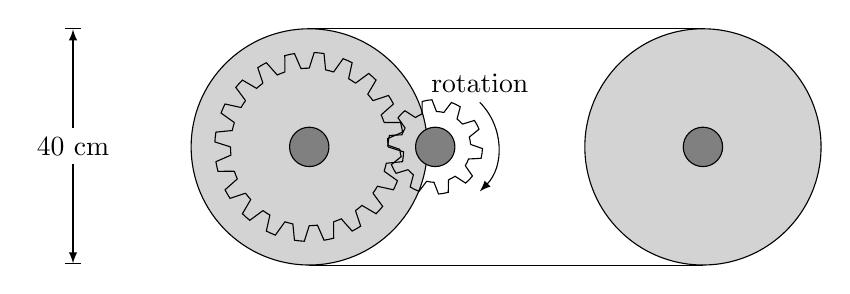
\begin{tikzpicture}[>=latex]
  \node[draw, circle, fill=LightGrey, minimum width=3cm](lpull){};
  \node[xshift=5cm, draw, circle, fill=LightGrey, minimum width=3cm](rpull){};
  \node at (rpull.center) [draw, circle, fill=Grey, minimum height=5mm]{};
  \draw (lpull.north) -- (rpull.north);
  \draw (lpull.south) -- (rpull.south);
  \draw [|<->|] (lpull.north) ++ (180:3) --++ (-90:3) node[midway, fill=White]{40 cm};
  \draw
  \foreach \i in {1,2,...,20} {%
    [rotate=(\i-1)*18] (0:1)  arc (0:6:1) -- (9:1.2)  arc (9:15:1.2) --  (18:1)
  };
  \node [draw, circle, minimum height=5mm, fill=Grey](shaft2){};
  \draw [xshift=1.6cm]
  \foreach \i in {1,2,...,10} {%
    [rotate=(\i-1)*36+4] (0:0.45)  arc (0:12:0.45) -- (18:0.6)  arc (18:30:0.6) --  (36:0.45)
  };
  \node [xshift=1.6cm, draw, circle, minimum height=0.5cm, fill=Grey](shaft1){};
  \draw [->] (shaft1.center) ++ (45:0.8) arc (45:-45:0.8) node[at start, above]{rotation};
\end{tikzpicture}
\caption{side view of conveyor assembly}
\end{figure}

\begin{figure}[H]
  \centering
  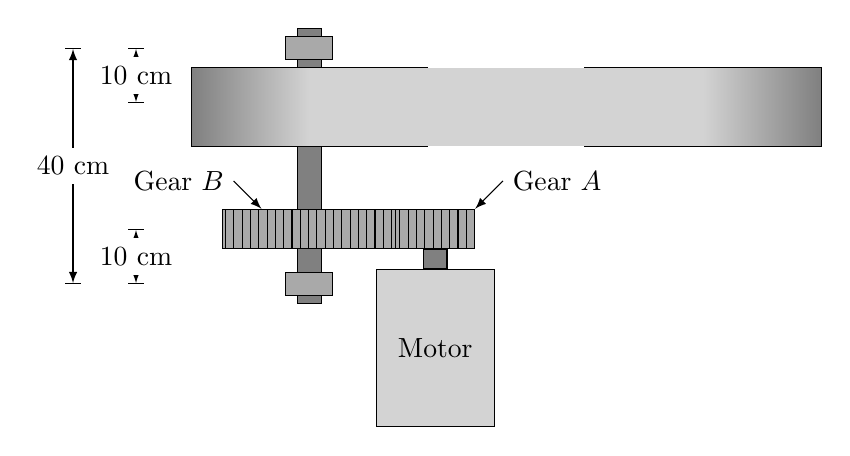
\begin{tikzpicture}[>=latex]
    \node [draw, fill=Grey, minimum width=3mm, minimum height=3.5cm](lshaft){};
    \node at (lshaft.north) [anchor=north, yshift=-5mm, draw, left color=Grey, middle color=LightGrey, minimum width=3cm, minimum height=1cm](lpull){};
    \node at (lshaft.north) [anchor=north, xshift=5cm, yshift=-5mm, draw, right color=Grey, middle color=LightGrey, minimum width=3cm, minimum height=1cm](rpull){};
    \node at (lpull.center) [anchor=west, fill=LightGrey, minimum width=5cm, minimum height=1cm]{};
    \node at (lshaft.north) [anchor=north, yshift=-1mm, draw, minimum width=6mm, minimum height=3mm, fill=DarkGrey](bearing1){};
    \node at (lshaft.south) [anchor=south, yshift=1mm, draw, minimum width=6mm, minimum height=3mm, fill=DarkGrey](bearing2){};

    %%%% Spur Gear B %%%%%%
    \node at (lshaft.south) [anchor=south, yshift=7mm, draw, minimum width=2.2cm, minimum height=5mm, fill=DarkGrey](gear2){};
    \node at (lshaft.south) [anchor=south, yshift=7mm, draw, minimum width=2.2cm, minimum height=5mm, pattern=vertical lines](gear2){};
    \draw [<-] (gear2.north west) ++ (0:0.5) --++ (135:0.5) node[left]{Gear $B$};

    %%%% Spur Gear A %%%%%
    \node at (lshaft.south) [xshift=1.6cm, anchor=south, yshift=7mm, draw, minimum width=1cm, minimum height=5mm, fill=DarkGrey](gear1){};
    \node at (lshaft.south) [xshift=1.6cm, anchor=south, yshift=7mm, draw, minimum width=1cm, minimum height=5mm, pattern=vertical lines](gear1){};
    \draw [<-] (gear1.north east) --++ (45:0.5) node[right]{Gear $A$};

    %%%% Motor shaft %%%%%
    \node at (gear1.south) [anchor=north, draw, fill=Grey, minimum height=2mm, minimum width=3mm](inshaft){};

    %%%% Motor %%%%%
    \node at (inshaft.south) [anchor=north, draw, fill=LightGrey, minimum height=2cm, minimum width=1.5cm](motor){Motor};

    %%%% Dimension for Shaft %%%%%
    \draw [|<->|] (bearing1.center) ++ (180:3) --++ (-90:3) node[midway, fill=White]{40 cm};
    \draw [|<->|] (bearing1.center) ++ (180:2.2) --++ (-90:0.7) node[midway, fill=White]{10 cm};
    \draw [|<->|] (bearing2.center) ++ (180:2.2) --++ (90:0.7) node[midway, fill=White]{10 cm};
  \end{tikzpicture}
  \caption{top view of conveyor assembly}
\end{figure}
\end{example}
\begin{solution}

  \begin{enumerate}
    \item To determine the number of teeth of spur gear $B$, we need to determine the required pitch line velocity. The belt must be moving at 60 cm/s, which means the pulley must be rotating at
          \begin{align*}
            \omega_{\text{pulley}} &= \frac{0.6}{\pi (0.2)} \\
                                   &= \py{round(0.6/pi/0.2,2)} \text{ rev/s} = \py{round(0.6/pi/0.2*60,1)} \text{ rpm}
          \end{align*}

          since spur gear $B$ is mounted on the same shaft as the pulley, it must have the same $\omega$. The pitch line velocities on two meshing gears must be the same. Spur gear $A$ rotates at 500 rpm, therefore, the pitch radius of spur gear $B$ is

          \begin{align*}
            r_{B} &= \frac{\omega_{A} r_{A}}{\omega_{B}} \\
                       &= \py{round(500*2.5/57.3,1)}
          \end{align*}
          Its diameter, of course, is \py{2*round(500*2.5/57.3,1)} cm. Given that meshing gears must also have the same module, the number of teeth on $B$ is

          \begin{align*}
            m &= \frac{D_{\text{pitch,A}}}{z_{A}} = {5}{10} = 0.5 \\
              &= \frac{43.6}{z_{B}} \\
            z_{B} &= \py{43.6*2} \text{ teeth}
          \end{align*}

    \item Assuming no power loss, the power the belt-pulley system needs to transfer is $P = T\omega = 2(500)(2\pi/60) = \py{round(2*500*2*pi/60,1)}$ W. Required torque transfer of the belt is $T = P/\omega = 104.7/(57.3(2\pi/60)) = \py{round(104.7/57.3/2/pi*60,1)}$ N-m. The tension difference on the two side needs to be
          \begin{align*}
            T &= (F_{1} - F_{2})r_{\text{pulley}} \\
            F_{1} - F_{2} &= \frac{T}{r_{\text{pulley}}} = \py{round(17.4/0.2)} \text{ N}
          \end{align*}

          We can now write an equation to determine the thickness $b$ of the belt
          \begin{align*}
            \frac{F_{1} - F_{c}}{F_{2} - F_{c}} = e^{\mu \theta}
          \end{align*}
          Set $F_{1} = (F_{1})_{a} = bF_{a}C_{v}C_{p} = b(6000)(1)(0.7) = 4200b$, $F_{2} = F_{1} - 87 = 4200b - 87$, $\mu = 0.5$, $\theta = \pi$, $F_{c} = (\gamma/g)bt \omega^{2} r^{2} = (9500/10)b(0.0013)(0.95(2\pi))^{2}(0.2)^{2} = \py{round(9500/10*0.0013*(0.95*2*pi)**2*0.2**2,2)}b$

          \begin{align*}
            \frac{4200b - 1.76b}{4200b - 87 - 1.76b} = e^{0.5 \pi} \\
            b = 0.0261 = 2.61 \text{ cm}
          \end{align*}

    \item To design the shaft, we must first determine the loads on the shaft, which are exerted by spur gear $B$ and the pulley. Let us determine the load from each component.

          The load from the gear can simply be determined by

          \begin{align*}
            F &= \frac{T}{r \cos \theta} \\
              &= \frac{17.4}{(0.2)(\cos 20^{\circ})} \\
              &= \py{round(17.4/0.2/cos(radians(20)),1)} \text{ N}
          \end{align*}

          So the force exerted on the shaft by gear $B$ is 92.6 N in the direction 20$^{\circ}$ downward from the tangential line between the two gears.

          The load from the pulley is even simpler

          \begin{align*}
            F_{p} &= F_{1} + F_{2} = 4200(0.0261) + 4200(0.0261) - 87 \\
              &= \py{4200*0.0261+4200*0.0261 - 87} \text{ N}
          \end{align*}

          The force exerted on the shaft by the pulley is 132 N to the right.

          Now all we need is to determine the maximum bending moment on the shaft.

          %%%%%%%% Simplified Bending Moment Summation %%%%%%%%%%
          %%%%%%%% Forces are not really going in the same direction
          %%%%%%%% So the moments must actually be broken down first.
          %%%%%%%% But given this is an exam, let's cut the students,
          %%%%%%%% and myself, some slack.


          First, bending moment $M_{g}$ generated by force in the gear is
          \begin{align*}
            M_{g} &= \frac{F_{g}x(L-x)}{L} = \frac{92.6(0.1)(0.4-0.1)}{0.4} \\
                  &= \py{round(92.6*(0.1)*(0.4-0.1)/0.4,2)} \text{ N-m}
          \end{align*}

          Next, bending moment $M_{p}$ generaed by force on the pulley is
          \begin{align*}
            M_{p} &= \frac{F_{p}x(L-x)}{L} = \frac{132(0.3)(0.4-0.3)}{0.4} \\
                  &= \py{round(132*(0.1)*(0.4-0.1)/0.4,2)} \text{ N-m}
          \end{align*}

          %%%%%% Maximum bending moment definitely NOT in the middle
          %%%%%% since the problem is not symmetrical.
          The maximum bending moment occurs in the middle, where
          \begin{align*}
            M_{\max} &= (6.95 + 9.9)\frac{2}{3} \\
                     &= \py{round((6.95+9.9)*2/3,1)} \text{ N-m}
          \end{align*}

          The maximum torque is just the required torque transfer, which is $T$ = 17.4 N-m. We can now determine the required shaft size.

          \begin{align*}
            N_{s} &= \frac{S_{y}}{\sigma_{e}} \\
            2 &= \frac{300 \times 10^{6}}{\sqrt{ \left( \dfrac{4(11.2)}{\pi r^{3}} \right)^{2} + 3 \left( \dfrac{2(17.4)}{\pi r^{3}} \right)^{2} }} \\
            r &= 0.0054 = 5.4 \text{ mm}
          \end{align*}

    \item Since the problem is not symmetrical, we need to determine the bearing under the higher load. This happens to the bearing closer to the higher force, which is the pulley. Taking the other bearing as a fulcrum, the radial load in the bearing on the pulley side is

          \begin{align*}
            F_{r} &= \frac{132(3)}{4} + \frac{92.6(1)}{4} \\
                  &= \py{round((132*3+92.6)/4,1)} \text{ N}
          \end{align*}

          With $L = 9 \times 10^{7}$ and $K_{r} = 1$, $F_{e} = F_{r} = 122.2 = C$. This is smaller than the smallest bore which is 10mm for all series. We therefore should pick the smallest bore (10 mm) as our choice.
  \end{enumerate}
\end{solution}

%\nocite{*}

\backmatter{}

\printbibliography[heading=bibintoc]

\end{document}
